\chapter{Handling Data for training the model}\label{chapt:data}
[\textit{As stated before [in \ref{chapt:problem}], In this work report, I will be using images from setinel-2A.}]

\section{Get the raw training dataset}
Data needed for training the model is divided into two parts: (a) Satellite image and the (b) Labelled dataset of Roads. Both (a) and (b) should be from the same geography. \par

Satellite images for Sentinel-2A are available at \url{https://scihub.copernicus.eu/dhus/}. For deep learning, a very accurately labeled dataset is crucial for model training. The pixel-level dataset is difficult to produce in any small community. This is when the web-map services come into the picture. One of the popular mapping services: Open Street Map(OSM) has been widely used for finding the road vectors. I will use out satellite images with the road vectors obtained from OSM. An advantage of using OSM is a lot of manpower is saved, and the main work can be focussed on writing code to validate the research, thus making the process efficient.


\section{Converting data to a usable form}
Even after obtaining the satellite image and roads dataset for the same geographical area, the final result image is quite big for DCNN to handle. \ref{chapt:problem}. To solve this problem, I sliced the image into multiple images of size 544*544 (Figure~\ref{fig:run_split_images}). This results in multiple small images which can be handled well by a computer (16GB RAM). This size can be decreased or increased depending on the specifications of the computer used.

\begin{figure}[h!]
  \centering
  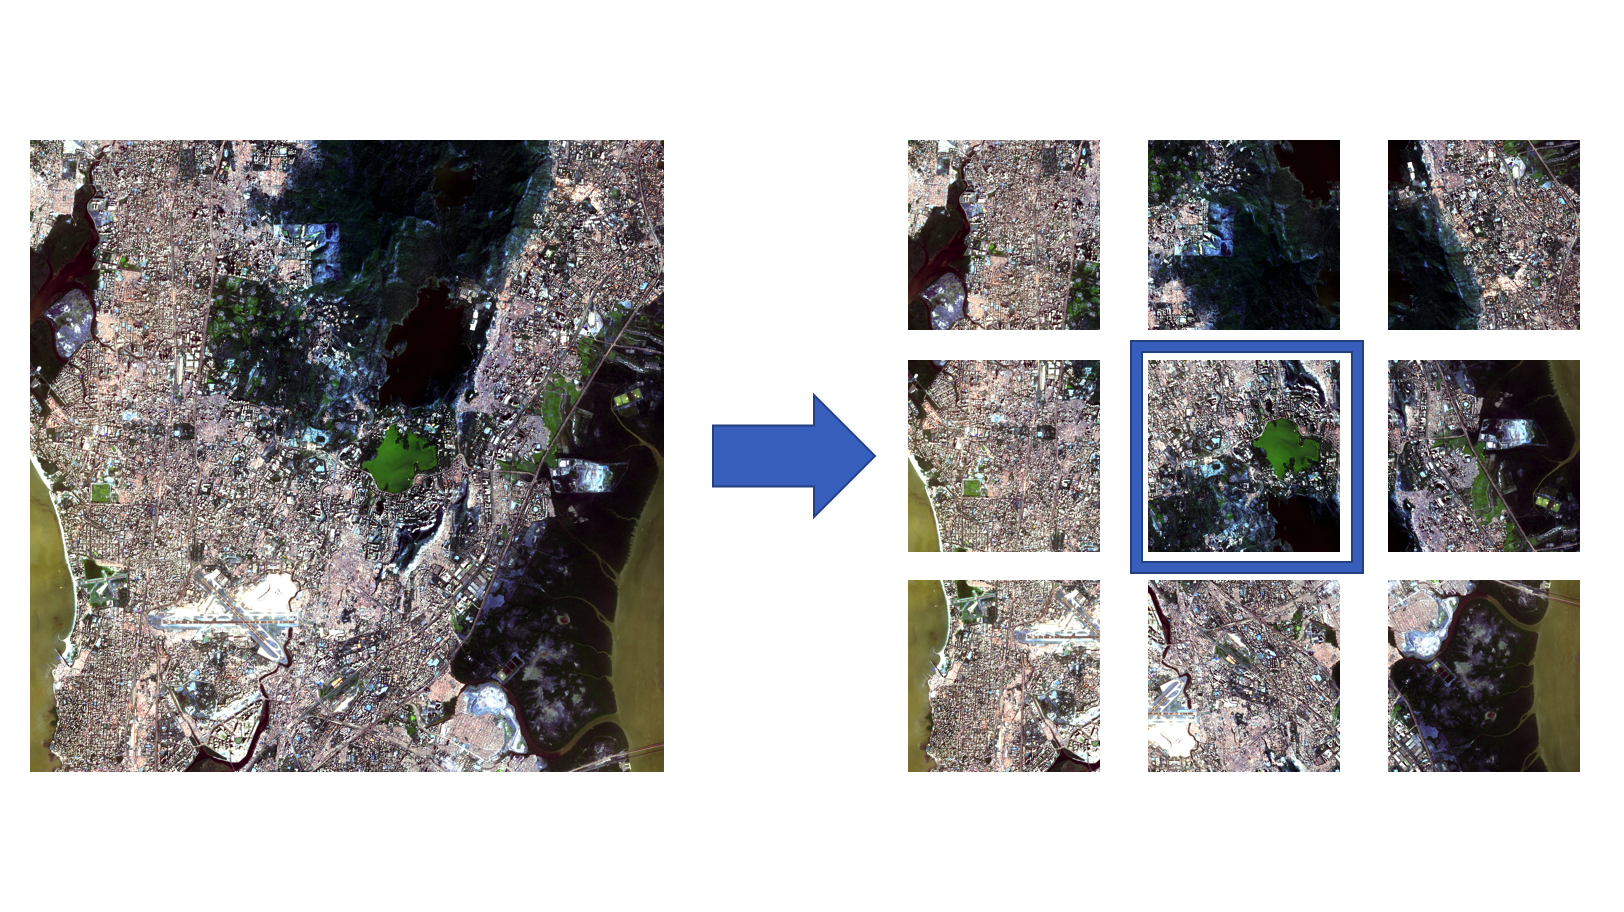
\includegraphics[height=60mm]{run_split_image}
  \caption{Image split into 9 parts making it fit for practical use in models.}
  \label{fig:run_split_images}
\end{figure}


\section{Cleaning the obtained dataset}
Though the data is from OSM by multiple collaborators, it is more or less in a crude format and prone to errors. Given it's open source in nature, It may be outdated or in some cases need some corrections. These corrections needs to be manually done to make sure the training data is accurate before being fed into our model. \par

The images with less or no roads are removed from the dataset. This is so that `the no road` data should not affect the weights which will be used to identify roads. This step is significant because roads often make up a very small part of satellite images, and most training images will have no roads on them. \par


\section{Handling pixel-level errors due to super-resolution}
While training the road-detection model, few unplanned errors prop up. Applying super-resolution results in generation of extra noise which disturbs the pixel-level accuracy of data. Due to errors in the intermediate data, the model might learn in some false values. This is reduced by use of a modified loss function applied during training of our road-detection model.